\section{The constant}\label{sec:constant}

We use the complete elliptic integrals of modulus $k\in[0,1)$,
\begin{gather*}
K(k)=\int_0^{\pi/2}\frac{\dd\phi}{\sqrt{1-k^2\sin^2\phi}},\\
E(k)=\int_0^{\pi/2}\sqrt{1-k^2\sin^2\phi}\,\dd\phi ,
\end{gather*}
and the moduli attached to the band,
\[
k=\sqrt{1-a^2/b^2},\qquad k'=a/b,\qquad
\kappa=\frac{b-a}{b+a}=\frac{1-k'}{1+k'} .
\]
The facts on $K$ and $E$ that we use are collected in \cref{app:elliptic}.

\begin{proposition}\label{prop:J}
With $I_0=\int_a^b\dd t/r(t)$ and $I_2=\int_a^bt^2\dd t/r(t)$,
\[
I_0=\frac{K(k)}b,\qquad I_2=b\,E(k),
\]
and
\begin{equation}\label{eq:J}
\begin{aligned}
J&=(a^2+b^2)I_0-2I_2=b\big[(1+k'^2)K(k)-2E(k)\big]\\
&=2(a+b)\big[K(\kappa)-E(\kappa)\big].
\end{aligned}
\end{equation}
Consequently
\begin{equation}\label{eq:Lambda-closed}
\Lambda=\frac{K(\kappa)-E(\kappa)}{\kappa}.
\end{equation}
\end{proposition}

\begin{proof}
Substitute $t^2=b^2-(b^2-a^2)\sin^2\phi$, $0\le\phi\le\pi/2$. Then
$b^2-t^2=(b^2-a^2)\sin^2\phi$, $t^2-a^2=(b^2-a^2)\cos^2\phi$,
$t\dd t=-(b^2-a^2)\sin\phi\cos\phi\dd\phi$, hence $\dd t/r(t)=-\dd\phi/t$ and
$t=b\sqrt{1-k^2\sin^2\phi}$. This gives $I_0$ and $I_2$, and the second form of
$J$. The Landen transformation (\cref{app:elliptic}) states
\[
K(k)=(1+\kappa)K(\kappa),\qquad E(k)=(1+k')E(\kappa)-k'K(k).
\]
Inserting these,\footnote{The coefficient of $K(\kappa)$ is $b(1+\kappa)\big[(1+k'^2)+2k'\big]=b(1+\kappa)(1+k')^2$, the term $2k'$ coming from $-2E(k)$.} and using $b(1+\kappa)=2b^2/(a+b)$ and $1+k'=(a+b)/b$,
\begin{align*}
J&=b(1+\kappa)(1+k')^2K(\kappa)-2b(1+k')E(\kappa)\\
&=2(a+b)\big[K(\kappa)-E(\kappa)\big].
\end{align*}
Dividing by $2(b-a)=2\kappa(a+b)$ gives \eqref{eq:Lambda-closed}.
\end{proof}

\begin{proposition}\label{prop:Lambda}
\begin{enumerate}
\item[(i)] With $c_n=\binom{2n}{n}4^{-n}$,
\[
\Lambda=\frac\pi2\sum_{n\ge1}\frac{2n}{2n-1}\,c_n^2\,\kappa^{2n-1}
=\frac\pi4\kappa\Big(1+\frac38\kappa^2+\frac{15}{64}\kappa^4+\cdots\Big),
\]
a series with positive coefficients;\footnote{By \eqref{eq:KEseries}, $K-E=\frac\pi2\sum_{n\ge1}c_n^2\big(1-\frac1{1-2n}\big)\kappa^{2n}$ and $1-\frac1{1-2n}=\frac{2n}{2n-1}$; dividing by $\kappa$ gives (i).} in particular $\Lambda$ increases with
$\kappa$, that is, with $b/a$.
\item[(ii)] For all $0<a<b$,
\[
\frac\pi4\,\frac{b-a}{b+a}\ <\ \Lambda\ \le\ \frac\pi4\,\frac{\kappa}{1-\kappa^2}
=\frac\pi{16}\,\frac{b^2-a^2}{ab}.
\]
\item[(iii)] As $a/b\to0$,
$\Lambda=\log\frac{4}{\kappa'}-1+o(1)=\frac12\log\frac{4b}{a}-1+o(1)$,
with $\kappa'=\sqrt{1-\kappa^2}=2\sqrt{ab}/(a+b)$.
\end{enumerate}
\end{proposition}

\begin{proof}
(i) From $K=\frac\pi2\sum c_n^2\kappa^{2n}$ and
$E=\frac\pi2\sum c_n^2\kappa^{2n}/(1-2n)$ one gets
$K-E=\frac\pi2\sum_{n\ge1}c_n^2\kappa^{2n}\,2n/(2n-1)$. The coefficients for
$n=1,2,3$ are $\frac12$, $\frac3{16}$ and $\frac{15}{128}$, which give the
displayed expansion after division by $\kappa$.
(ii) The lower bound is the first term. For the upper bound, the ratio of
consecutive coefficients $d_n=c_n^2\,2n/(2n-1)$ is
\[
\frac{d_{n+1}}{d_n}=\frac{(2n+1)(2n-1)}{(2n+2)\,2n}<1,
\]
so $d_n\le d_1=\frac12$ and $K-E\le\frac\pi4\sum_{n\ge1}\kappa^{2n}
=\frac\pi4\kappa^2/(1-\kappa^2)$. Finally $\kappa/(1-\kappa^2)=(b^2-a^2)/(4ab)$.
(iii) As $\kappa\to1$, $K(\kappa)=\log(4/\kappa')+o(1)$ and $E(\kappa)\to1$
(\cref{app:elliptic}); and $\log(4/\kappa')=\log\big(2(a+b)/\sqrt{ab}\big)
=\frac12\log(4b/a)+o(1)$.
\end{proof}

For a narrow band with centre $\bar\omega=(a+b)/2$ and width
$\Delta\omega=b-a$, $\kappa=\Delta\omega/(2\bar\omega)$, so
\begin{equation}\label{eq:narrow}
\Lambda=\frac\pi8\,\frac{\Delta\omega}{\bar\omega}
\Big(1+O\big((\Delta\omega/\bar\omega)^2\big)\Big).
\end{equation}
The bound is linear in the relative bandwidth, which is what one expects: on
an infinitely narrow band a delay achieves any phase without loss. For wide
bands it grows only logarithmically in $b/a$. \Cref{tab:lambda} gives values,
also in decibels per degree of phase, which is $\Lambda$ times
$(20/\ln 10)(\pi/180)=0.15160$, and \cref{fig:bound} shows the bound as a
surface.

\begin{table}[t]
\caption{The constant $\Lambda$ of \eqref{eq:Lambda-closed}, the least mean
attenuation per radian of constant phase lag, for several band ratios. The
last column is the least worst-frequency power loss for $\theta=1^\circ$.}
\label{tab:lambda}
\centering
\small
\begin{tabular}{@{}rrrrr@{}}
\toprule
$b/a$ & $\kappa$ & $\Lambda$ (Np/rad) & dB/deg & $1-e^{-2\Lambda\pi/180}$ \\
\midrule
$1.01$ & $0.004975$ & $0.003907$ & $0.000592$ & $1.36\times10^{-4}$\\
$1.1$  & $0.04762$  & $0.03743$  & $0.00567$  & $1.31\times10^{-3}$\\
$1.5$  & $0.2$      & $0.1595$   & $0.0242$   & $5.55\times10^{-3}$\\
$2$    & $0.3333$   & $0.2735$   & $0.0415$   & $9.50\times10^{-3}$\\
$3$    & $0.5$      & $0.4366$   & $0.0662$   & $1.51\times10^{-2}$\\
$10$   & $0.8182$   & $0.9448$   & $0.143$    & $3.24\times10^{-2}$\\
$100$  & $0.9802$   & $2.016$    & $0.306$    & $6.80\times10^{-2}$\\
$1000$ & $0.9980$   & $3.150$    & $0.478$    & $1.04\times10^{-1}$\\
\bottomrule
\end{tabular}
\end{table}

\begin{figure}[t]
\centering
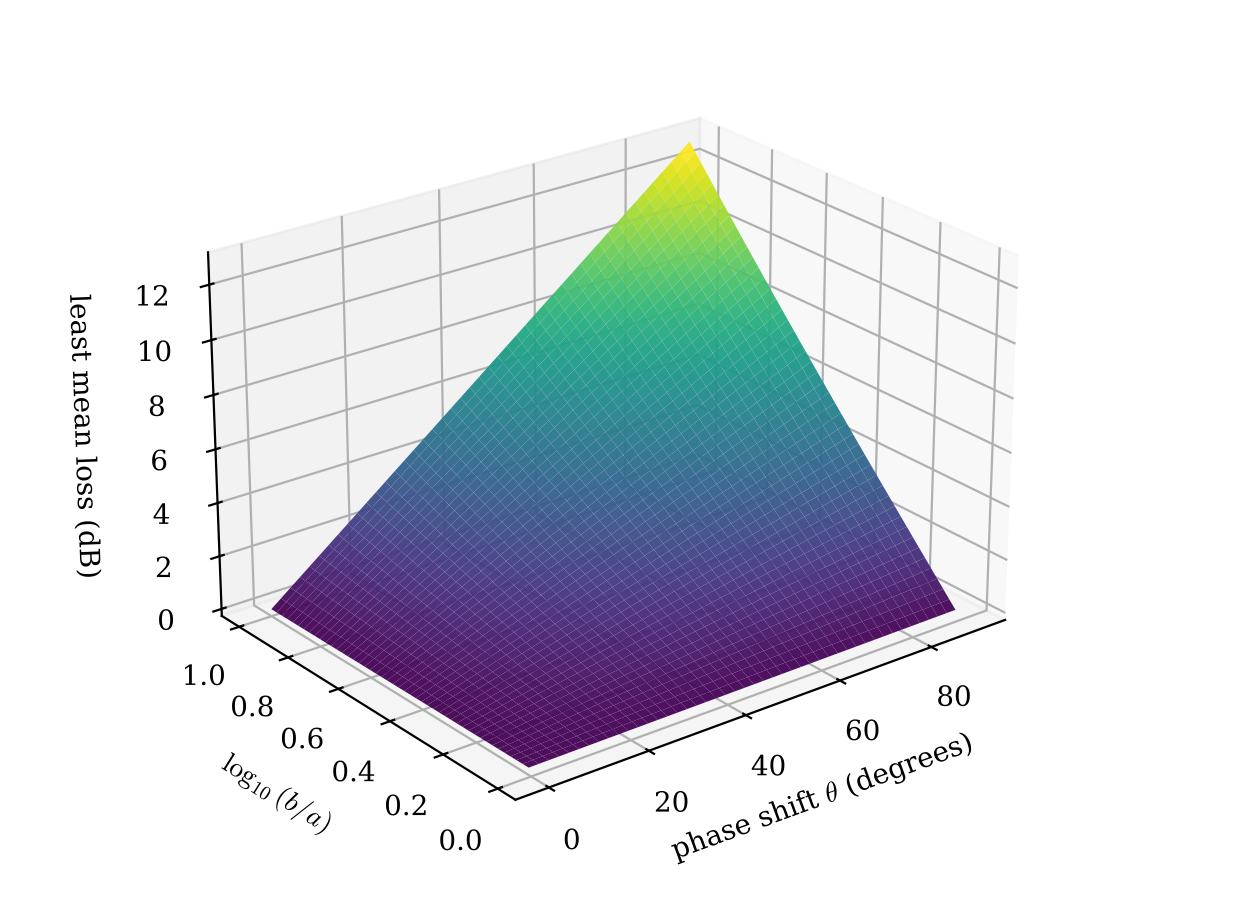
\includegraphics[width=\columnwidth]{figures/fig_bound.png}
\caption{The least mean loss $\theta\Lambda$, in decibels, over the phase lag
$\theta$ and the band ratio $b/a$. The surface is linear in $\theta$ and
increasing in $b/a$.}
\label{fig:bound}
\end{figure}
